% !TEX root = ../Thesis.tex
% !TEX spellcheck = en-US

\chapter{Kathará}
\label{ch:kathara}

In this chapter, we present Kathará in further detail.
Its structure is as follows: in the first section, Kathara's functional capabilities are described from a high-level vantage point, as well as its user interface; then follows a lower-level explanation of this emulation framework's architecture and implementation; finally, a case study identical to the one applied to GNS3 on section~\ref{sec:gns3practicalcasestudy} is presented.

% As said before, Kathará is a new implementation of Netkit, done from the ground up, which shares the same declarative language for preconfiguring labs (both the topology in terms of nodes and ``links'', as well as the default behavior and configuration of each node) with the latter, using an almost identical command-line interface.

% Despite having being developed to deploy very different kinds of networks than those of Netkit, namely software-defined networks, those with programmable data plane nodes, and with virtual network functions, Kathará is recommended as a successor by its precursor's website, since it promises total backwards compatibility, while having a more portable and efficient architecture, thanks to relying on Docker.

% Section "UI and functionality"
\section{UI and Functionality}
\label{sec:katharafunctionality}

% To build such a framework, the chosen starting point was an experimental tool called sdnetkit, which enhanced Netkit with OpenFlow enabled switches, still explicitly supporting ``traditional routers'' performing distributed routing protocols like OSPF~\cite{sdnkit}.
% Kathará then evolved to be a fully backwards compatible tool with Netkit, using the same conceptual philosophy in terms of interfaces and emulated topology definition, with a substantially different implementation, and the capabilities mentioned earlier in this section.

The high-level functional capabilities of Kathará explored in this work are the exactly the ones shared with the original Netkit---i.e. building and emulating topologies with traditional routers and switches and generic hosts.
However, as will be seen later, the implementation changes and overall modernization that Kathará brings can benefit any user.

As a side-note, it's important to point out that Kathará officially provides a very comprehensive repository of hands-on labs,\footnote{\mbox{\url{https://github.com/KatharaFramework/Kathara-Labs}}} mostly in the form of a PDF containing a sequence of slides and an archive with a shareable Kathará lab with part of the work done, so that many didactic topics in networking, from traditional routing to \gls{sdn}, NFVs, and ``behavioral model'' (P4 language), can be followed step-by-step, with some theory in the middle.
The first one of those ``labs'' is the `Introduction to Kathará,' referred to afterwards.

% Figure fig:kathara-topologynodes
\begin{figure}
  \centering
  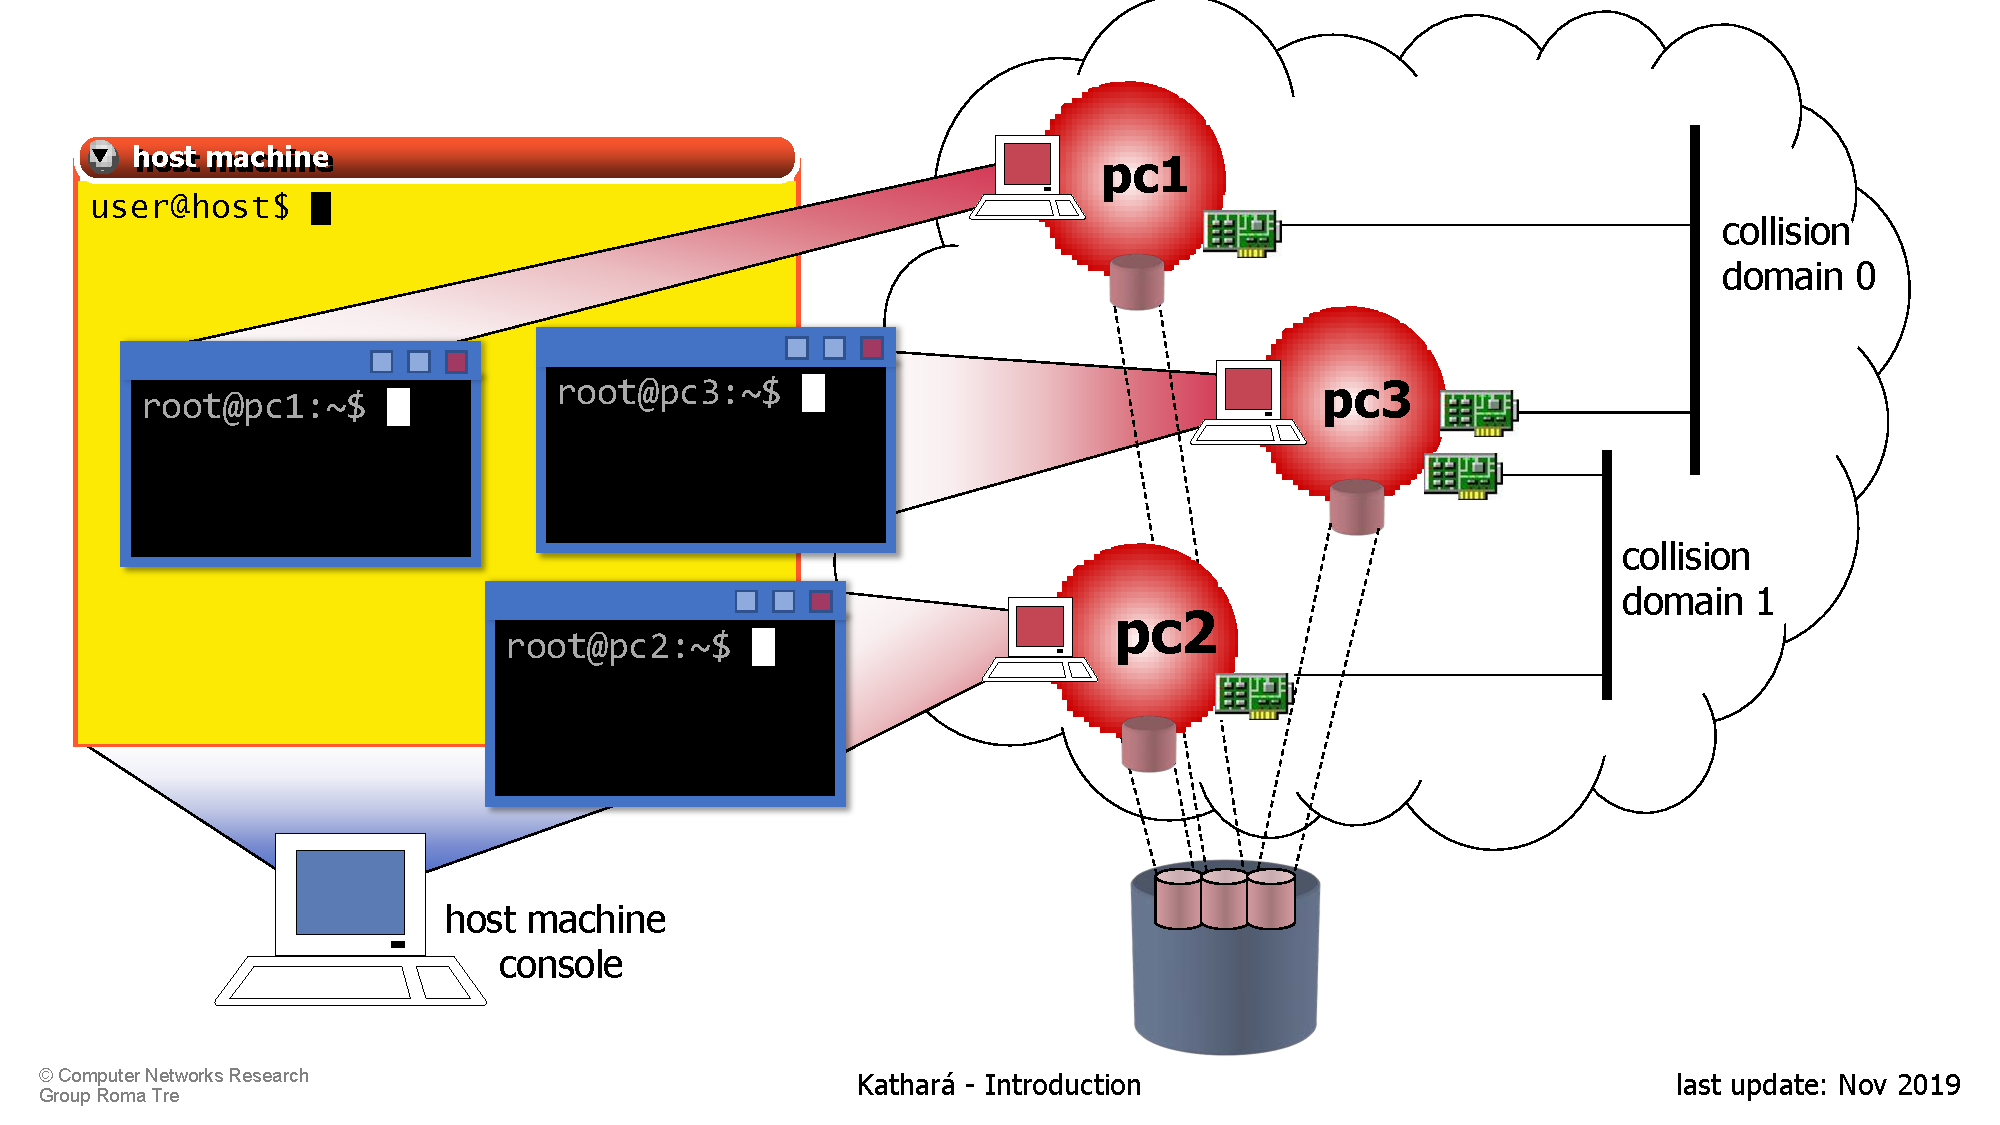
\includegraphics[width=0.8\textwidth,frame]{kathara-topologynodes}
  \caption{Slide taken from `Introduction to Kathará' showing a simplified lab in action}
  \label{fig:kathara-topologynodes}
\end{figure}


As stated in `Introduction to Kathará,' each (emulated) device has:
\begin{itemize}
  \item a console (a terminal window) which gives access to a \texttt{bash} shell inside the container
  \item an (virtually) isolated memory
  \item an (virtually) isolated filesystem, though Kathará provides a way to mount shared files among the nodes of the lab, via a convention of directory hierarchies so no explicit configuration is needed
  \item zero, one, or more network interfaces
\end{itemize}

The slides also explain that each network interface can be connected to a (virtual) collision domain and each virtual collision domain can be connected to several interfaces.
All this is illustrated by figure~\ref{fig:kathara-topologynodes}.

Kathará's interface has two parts: a set of commands that can be issued in the host (the machine where the emulator is being executed) shell, and the a structured way to define labs, which includes a syntax for defining topologies---i.e. which nodes are there, what are their names, how many network interfaces do they have and to which collision domain (i.e. links) are they connected to---and also a conventionalized way to structure configuration files that are automatically read by the software inside the nodes, like IP configurations or routing parameters.

These interfaces are not exhaustively exposed in this work since that would just mean duplicating the documentation resources, which are easily accessible and very clear.
However, figure~\ref{fig:kathara-topologynodes} serves as a way to illustrate, in contrast with graphical interactive tools, the way topologies are described and allows to take an immediate conclusion: to have only point-to-point links, this means that only each two interfaces that are connected via that each link need a separate collision domain and local-area networks of interconnected $N$ Ethernet-equiped hosts need a switch between them.

What was just said poses a question that will be further explored in the practical case study (section~\ref{sec:katharapracticalcasestudy}): there aren't conventional (layer-2) switching labs in the aforementioned repository, and the routing ones assume that more than one hosts sharing the same IP-prefix simply share collision domains.

% Figure fig:kathara-topologynodes
\begin{figure}
  \centering
  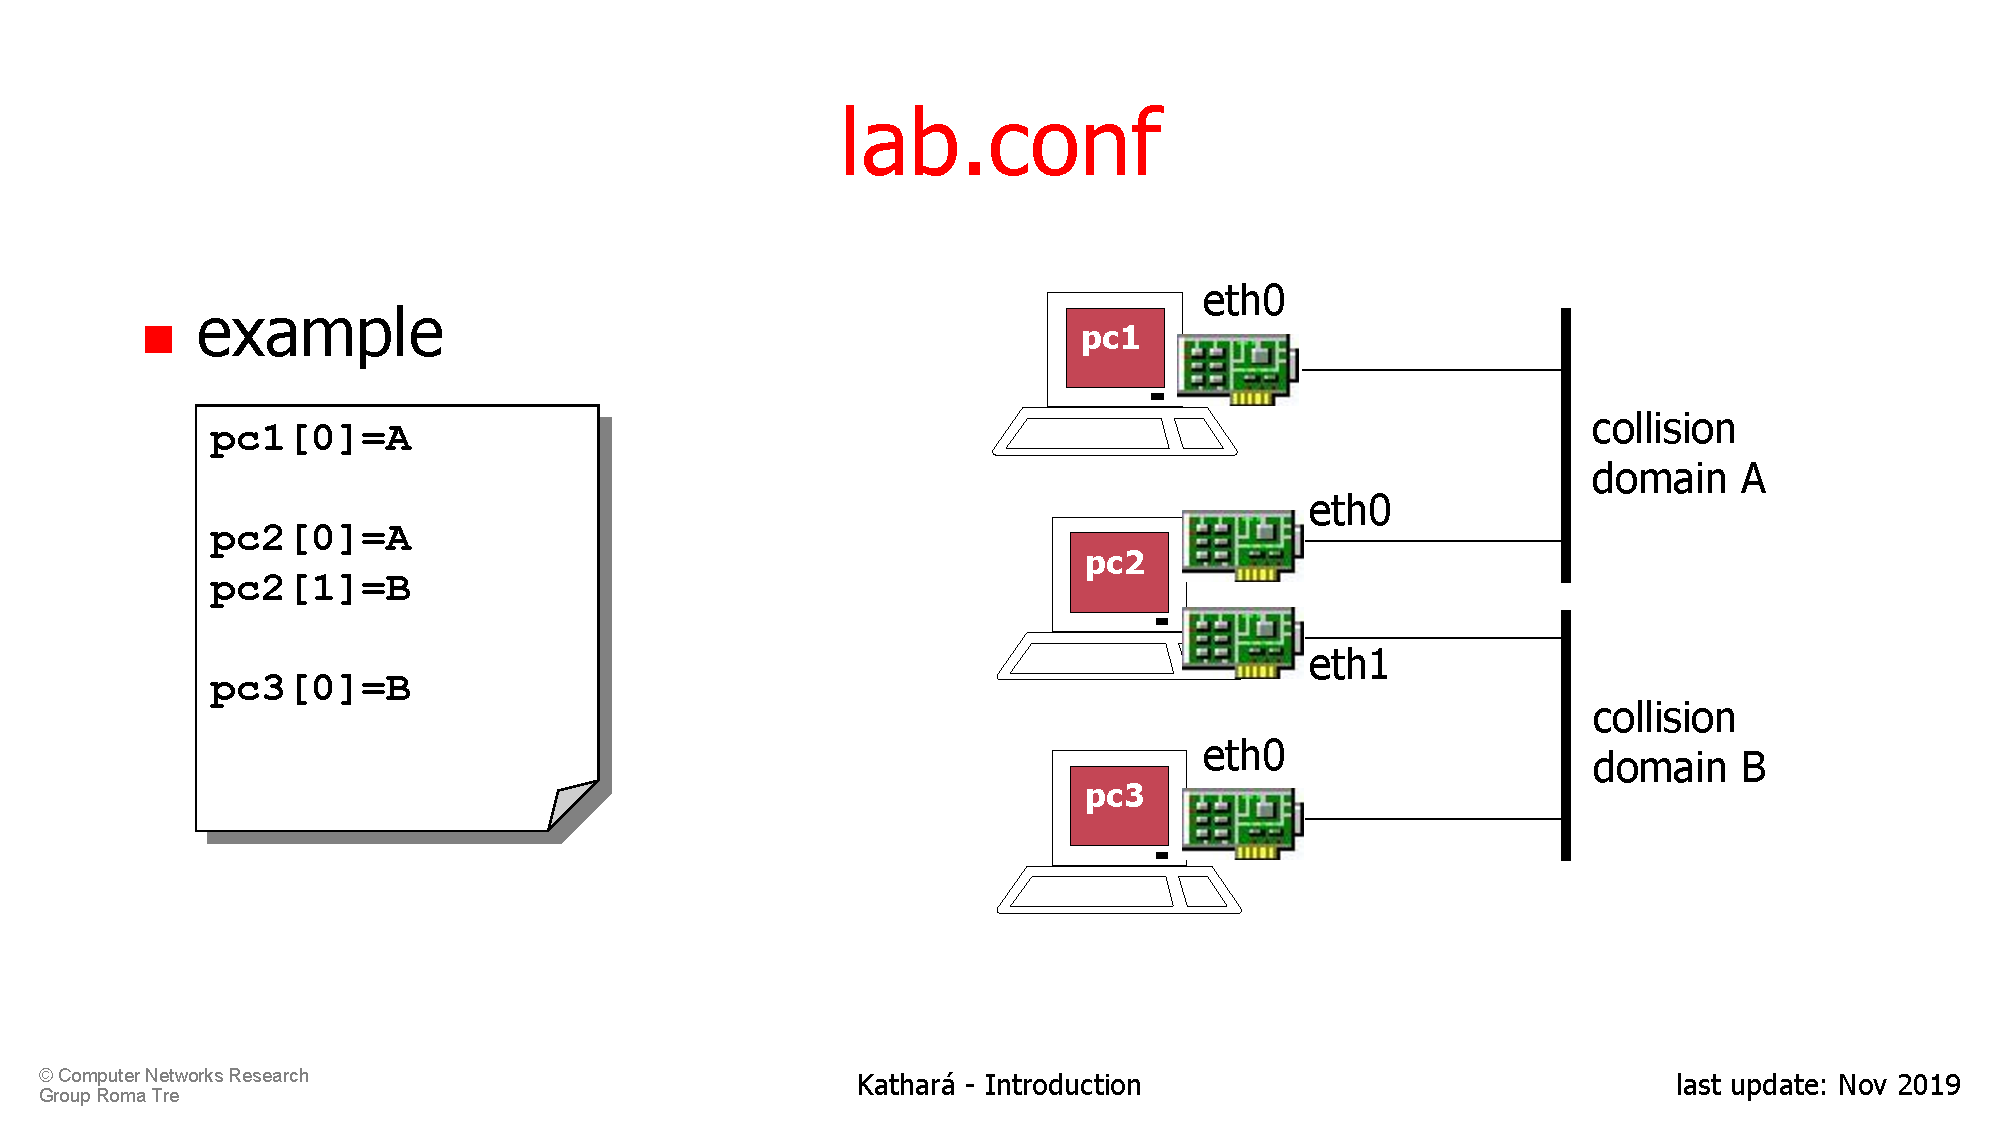
\includegraphics[width=0.8\textwidth,frame]{kathara-labconf}
  \caption{Slide taken from `Introduction to Kathará' showing the mapping between \texttt{lab.conf} and the instantiated topology}
  \label{fig:kathara-labconf}
\end{figure}


% end of section katharafunctionality


% Section "Technical overview"
\section{Technical Overview}
\label{sec:katharatechnicaloverview}

In Kathará's original announcement's paper~\cite{kathara}, the described technical infrastructure of the program, which can easily be confirmed by consulting the available Python source code,\footnote{\mbox{\url{https://github.com/KatharaFramework/Kathara}}} clearly states the basic design decision that follows the choosing of lightweight containers via Docker: every node in the topology is a Docker container.
Kathará, therefore, works as an orchestrator of containers, the same way that Docker's own Compose\footnote{\textquote{Compose is a tool for defining and running multi-container Docker applications \ldots\ with a single command, you create and start all the services from your configuration.}~\mbox{\url{https://docs.docker.com/compose/}}} is.
The difference is that, while Docker Compose exposes a limited set of network parameterization, given that its purpose is to handle the combination of different application-level services running in containers that must be able to exchange IP traffic between each other, Kathará uses lower-level primitives exposed by Docker itself to setup the containers' virtual interfaces and hook them up to virtual collision domains which serve as a shared medium between any number of nodes, and therefore constitute links or hubs in a topology.

% Figure fig:kathara-architecture-paper
\begin{figure}
  \centering
  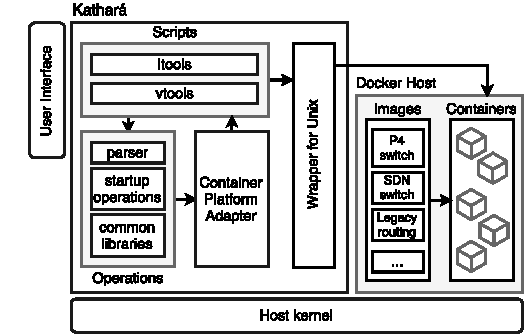
\includegraphics[width=0.8\textwidth]{kathara-architecture-paper}
  \caption{The diagram where Kathara's authors present its architecture}
  \label{fig:kathara-architecture-paper}
\end{figure}


Kathará's own architecture, depicted in figure~\ref{fig:kathara-architecture-paper}, is decribed as comprising three parts:
% Scripts, Operations, and Container Platform Adapter
\begin{description}
  \item[Scripts] used by the users to interact with Kathará.
  These scripts implement the basic operations that are used to start, stop, and pause the network nodes defined in the Kathará configuration and are divided into the two categories referred to in section~\ref{sec:katharafunctionality}, the \texttt{ltools} and the \texttt{vtools}.
  \item[Operations] is a module which \textquote{includes a set of utility functions that are used by the Scripts module in order to allow Kathará to interpret the configuration provided by the users.}
  This module is made of three main logical components: \emph{parser}, \emph{start-up operations}, and \emph{common libraries}.
  The parser is responsible by translating the textual configuration into a network topology; the start-up operations component ensures the cross-system compatibility, namely copying the files that must be copied to inside the nodes;
  \item[Container Platform Adapter] is a layer between the Operations module and Docker, which could allow to use different container platforms other than Docker.
\end{description}

To separate different kinds of nodes with different specific needs in terms of the software (e.g. daemons available to be run) running on them, Kathará allows for its topologies to specify which Docker image it should be running.
The default one (which can be changed on the program's preferences) is \texttt{kathara/quagga}. Therefore, all nodes, are able to launch any of Quagga's functionality, even if they, by omission, don't do it.
For P4 or \gls{sdn} enabled switches, two different images exist, as well as for the ClickOS-enabled one for creating \glspl{vnf}.

The Docker networking mechanism~\cite{dockernetworking} to create the collision domains through which interfaces of different containers communicate with each other is not explicitly stated in Kathara's paper.
Therefore, to be sure, one would need to look into the corresponding module on Kathara's source code.

% Kathará also leverages the notion of Docker images, available via Docker Hub or just setup locally on the user's Docker installation, both for separating the functionality (and ``role'') that different kinds of nodes may have on a lab (from being a traditional router to an OpenFlow switch, or an end-host running a RDBMS). % TODO first, take this out of here (maybe to the practical case study, when mentioning the way to create an inherited image), then add RDBMS to the acronyms

% end of section katharatechnicaloverview


% Section "Using Kathará. Practical case study"
\section{Using Kathará. Practical Case Study}
\label{sec:katharapracticalcasestudy}

For the practical case study of Kathará, we followed the same approach than for GNS3's, used the same laboratory handouts from APRC as reference, but implemented in Kathará's different paradigm.
Refer to section~\ref{sec:gns3practicalcasestudy} for an overview of the labs and their topics.

\subsection{Setting Topologies in Kathará}

As mentioned earlier in this chapter, Kathará doesn't offer a graphical interface to draw topologies, and nodes added and removed, started and stopped, and text-based consoles to them are created via a set shell commands.

We mentioned as well that, in Kathará, there aren't end-to-end links as such, like there are on GNS3.
Instead, Kathará has collision domains, which are Ethernet media, shared by whichever interfaces are attached to them, and all hosts connected through a collision domain can have packets sent back and forth among each other.
For instance, each IP-prefix corresponding to a logical LAN, connected to a layer-3 router, can have all its hosts attached to the same collision domain.

In spite of the aforementioned, to be coherent with what was done in the GNS3 case-study and to be able to compare both frameworks more fairly---and because it is a condition to perform the switching assignment, in lab handout~2---it was decided that we would always use point-to-point links, which in practice means creating as many collision domains as there are links, and attaching each corresponding pair of interfaces in the nodes to every correct one. % TODO este point-to-point está certo?

% Figure fig:kathara-annotated-lab3-topology
\begin{figure}
  \centering
  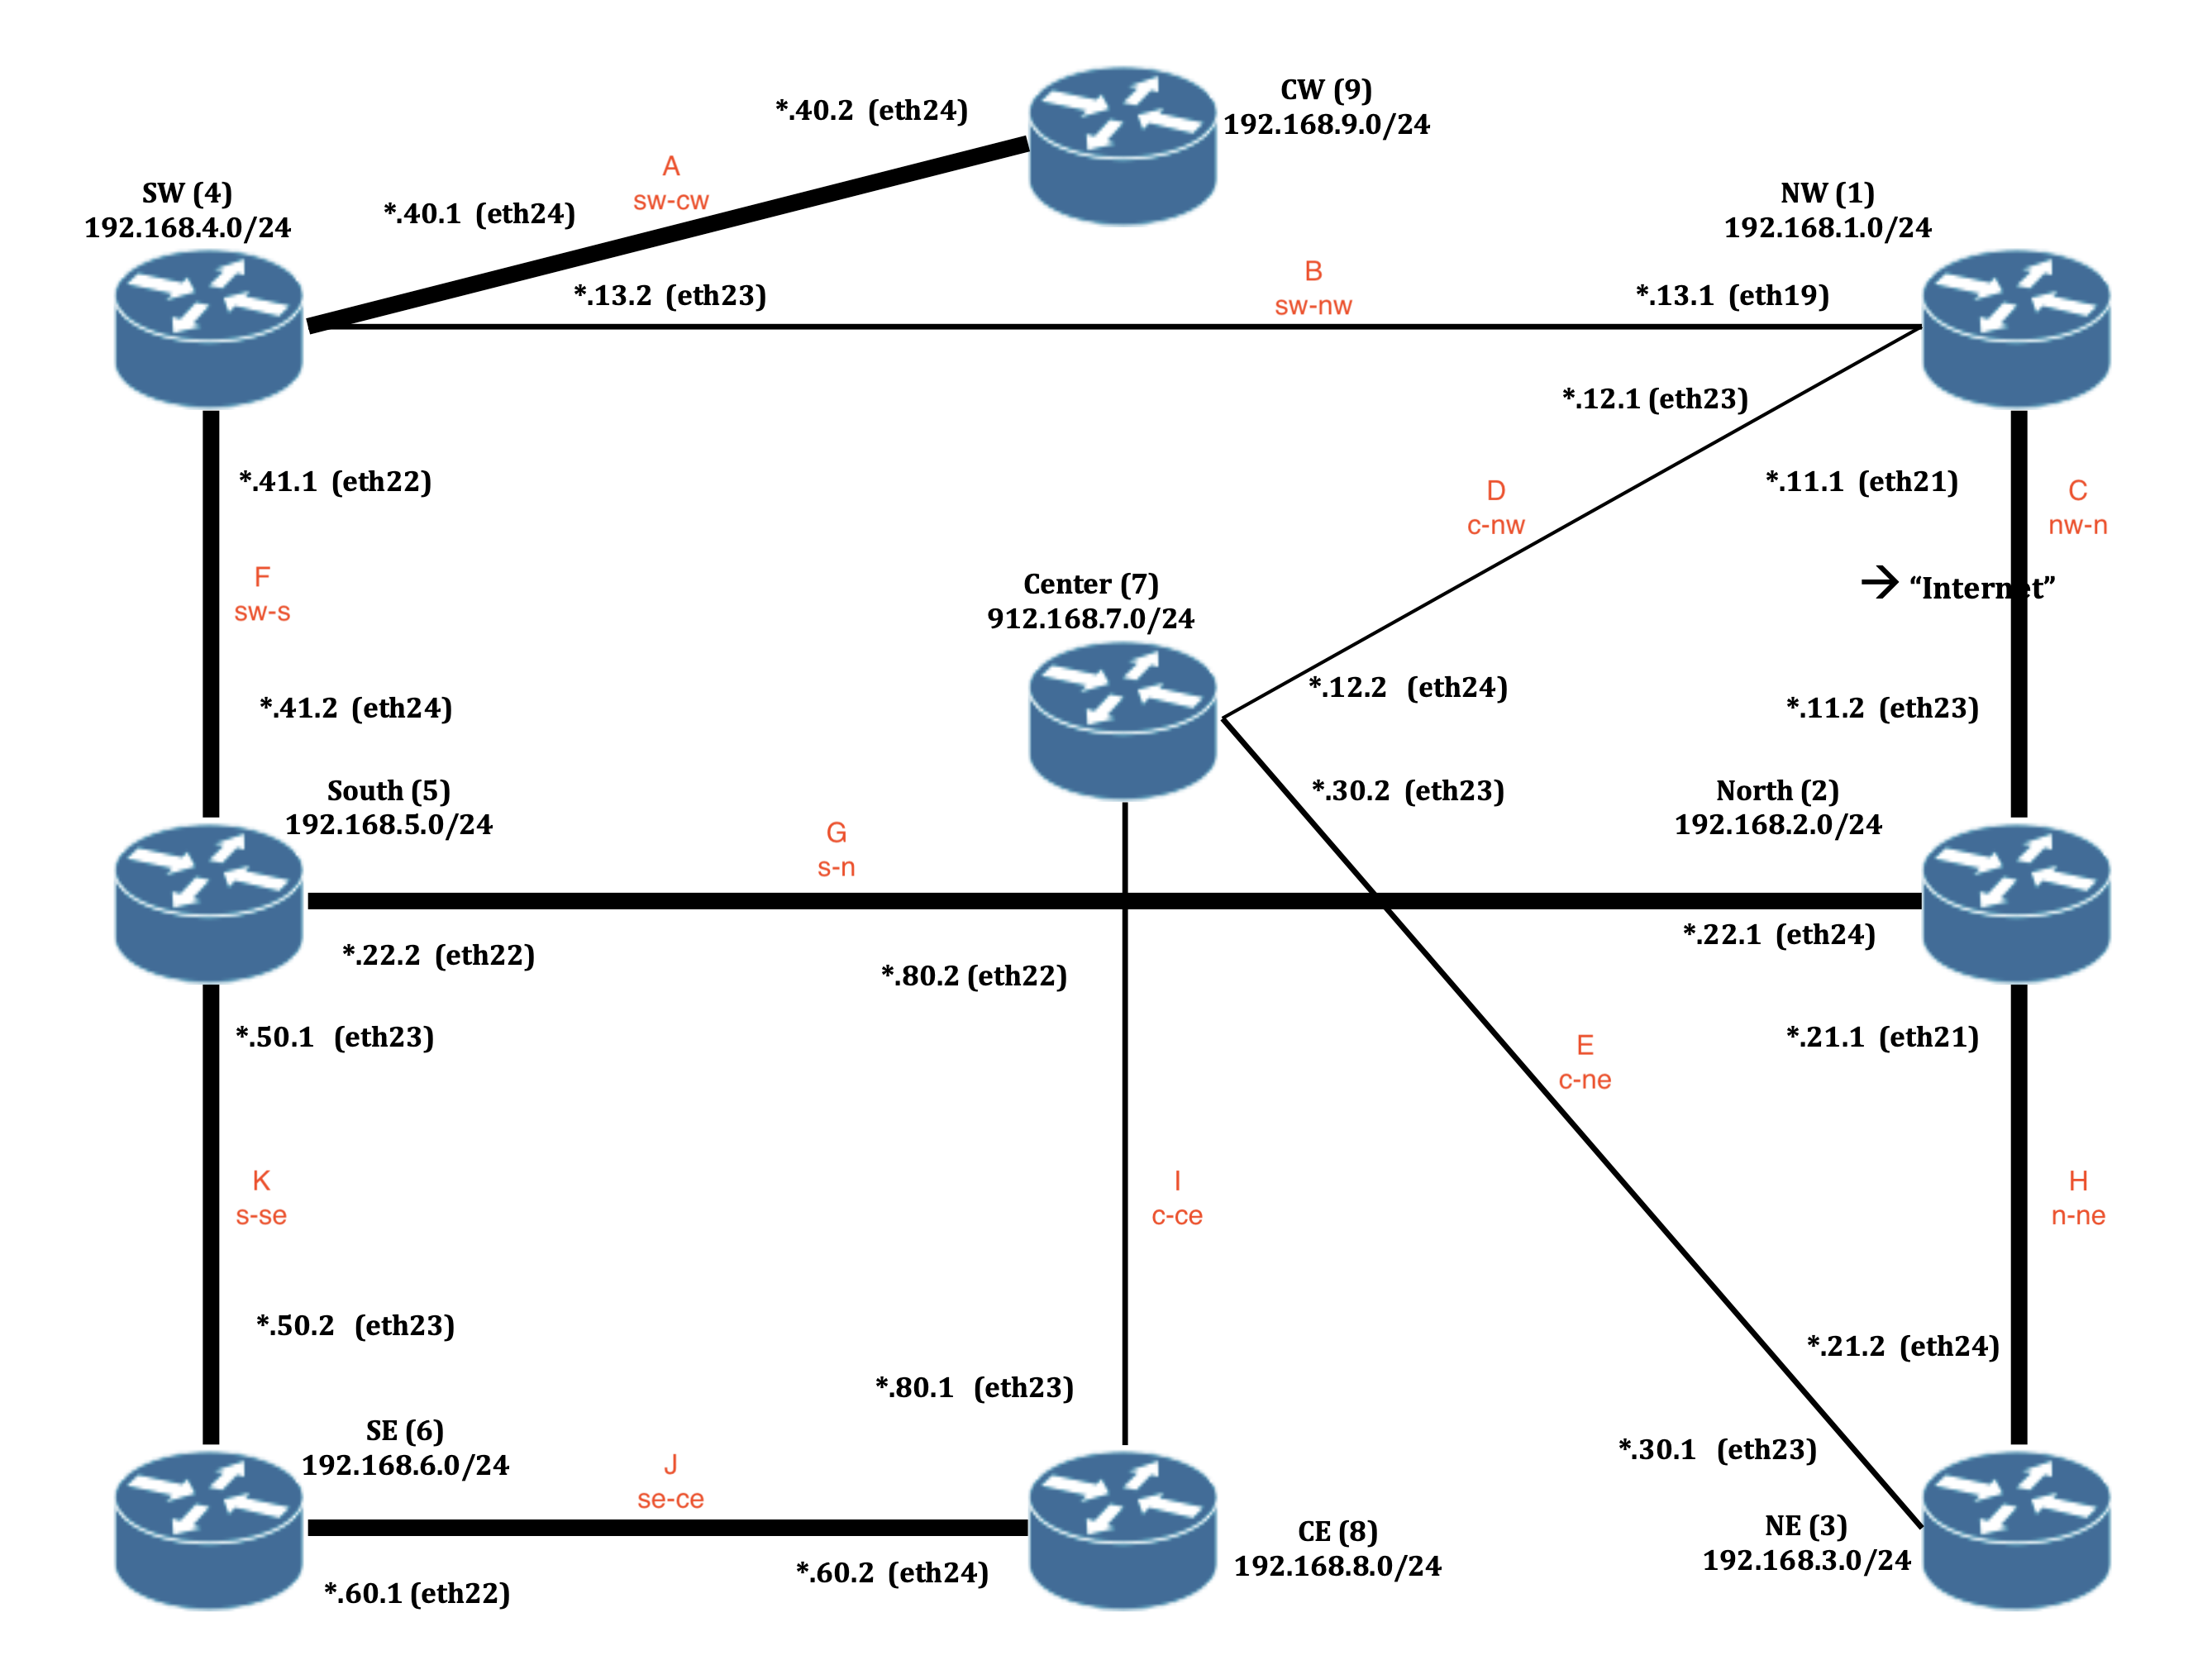
\includegraphics[width=\textwidth]{kathara-annotated-lab3-topology}
  \caption{Section of ``lab-assignment3'' showing the topology, with every collision domain annotated}
  \label{fig:kathara-annotated-lab3-topology}
\end{figure}


To facilitate this process, the graphical representation of the topology as given in the course's handout PDF was annotated with the letters that are becoming each collision domain, as figure~\ref{fig:kathara-annotated-lab3-topology} depicts. % TODO fazer versão vectorial desta figura
Then, writing Kathará's \texttt{lab.conf} and making sure that it is correct becomes much easier.

\subsection{Switching Exercises}

The switching lab was set up using a similar methodology than the one described just before for lab~3---i.e. the topology was graphically annotated to define the collision domains among the several interfaces.

Then, using Kathará's convention to ``pass-on'' configuration directories to each container, we defined the startup file (that is executed by its respective container when it ``boots up'') to setup a bridge virtual interface, according to the Linux bridge documentation and online resources~\cite{brctlman,howtobridgelinux}.

The configurations, both the \texttt{lab.conf}, which defines the topology, and one of the nine (the other ones are analogous and only vary in the number of interfaces) \texttt{<node\_name>.startup}, are shown as examples in the listings appendix as listings~\ref{listlab2conf} and~\ref{listlab2startup}, respectively.

For the switching exercises, we found out that there is some kind of limitation, either in Docker itself, in Docker's chosen intercontainer networking strategy, or in Kathará's implementation.
The containers (lightweight virtual Linux hosts), equipped with multiple \glspl{nic} that perform each switch, are not capable of successfully performing the Spanning Tree Protocol, which is demanding for a topology with a loop, which the exercise deliberately has.
We were not able to find a convincing explanation for this fact.

\subsection{Working Under Load and Version Control}

Kathará doesn't provide any \textbf{load balancing} mechanism out of the box.
Containers are expected to run under one single Docker host.
On the one hand, one can try to imagine ways to tunnel the traffic from certain nodes to any arbitrary different topology, by bridging virtual Docker interfaces to some of the hosts' interface.
On the other hand, as exposed in more detail later on, Kathará doesn't demand nearly as many resources for a large topology as GNS3.

Regarding \textbf{version control} (what, in GNS3, is achieved via \textbf{snapshots}), Kathará's approach is different.
Every relevant configuration is expected to be written, either in the configurations passed in conventionalized sub-directories of the project to the hosts to configure the routing daemons or any other software running in the container, or in the declaration of the graph in the \texttt{lab.conf}.
All of these are plain-text files, therefore the user is encouraged to resort to a version-controls solution, like Git\footnote{\url{https://git-scm.com}}.

\subsection{Performance measurements}

For completeness, we measured the host to host bandwidth in Kathará, measured with \texttt{iperf3}, like shown, in the case of GNS3, in~\ref{tab:gns3-iperf}.
The values are consistently~$\approx 25.0~\mbox{Gbit/s}$, even on 1~Gbps virtual \glspl{nic}.

A measure of the OSPF convergence time for this emulator was not performed.

% end of section katharapracticalcasestudy


% Section "Summary"
\section{Summary}
\label{sec:katharasummary}

This chapter presented Kathará as an emulator:
\begin{itemize}
  \item optimized for a use in academic environments, where vendor-specific aspects are not particularly relevant, only the implementation of protocols and networking functionality;
  \item very little resource-hungry due to its reliance on Docker containers, which are lightweight by nature;
  \item which offers a declarative, textual interface, both for topology definition and default node configuration, as well as interaction with an emulation in execution, through shell commands;
  \item able to very large topologies in one single host.
\end{itemize}

% end of section gns3summary


% end of chapter
